% AER-Article.tex for AEA last revised 22 June 2011

% \documentclass[AER]{AEA} modified for the full path to my AEA.cls file
\documentclass[AER]{./aea-latex-templates/AEA}

\usepackage{tikz}
\usetikzlibrary{calc,matrix}

% The mathtime package uses a Times font instead of Computer Modern.
% Uncomment the line below if you wish to use the mathtime package:
% \usepackage[cmbold]{mathtime}
% Note that miktex, by default, configures the mathtime package to use commercial fonts
% which you may not have. If you would like to use mathtime but you are seeing error
% messages about missing fonts (mtex.pfb, mtsy.pfb, or rmtmi.pfb) then please see
% the technical support document at 
% for instructions on fixing this problem.

% Uncomment the next line to use the harvard package with bibtex
\usepackage[abbr]{harvard}

% This command determines the leading (vertical space between lines) in draft mode
% with 1.5 corresponding to "double" spacing.
\draftSpacing{1.5}

% allowing images as figures
% ref: https://tex.stackexchange.com/questions/19176/how-to-insert-an-image-into-latex-document
\usepackage{graphicx}
\graphicspath{{./figures-and-tables}}

\begin{document}

\title{Attitudinal Trends in Alternative Postsecondary Learning}
\shortTitle{Trends in Alternative Learning}
\author{John Vandivier\thanks{Vandivier: George Mason University, 4400 University Dr, Fairfax, VA 22030, jvandivi@masonlive.gmu.edu. The author acknowledges valuable input from Bryan Caplan at George Mason University.}}
\date{\today}
\pubMonth{Month}
\pubYear{Year}
\pubVolume{Vol}
\pubIssue{Issue}
\JEL{D12, I21, I22, I24, I25, I26}
\Keywords{Education economics, alternative education, debt crisis, signaling}

\begin{abstract}
Traditional postsecondary learning in the United States is associated
with increased earnings and employment, but these benefits come at
substantial cost. Nontraditional education provides a partial workaround
with a variety of caveats including nonconformity stigma. This paper
explores a novel data set (n = 1190) to understand trends in public
disposition on alternative credentials. Results indicate that
favorability is high, declining in the short term, and may reverse trend
over time. Leveraging alternative pathways to reduce cost and accelerate
completion of accredited education is a recommended strategy. Some
policy considerations are discussed.
\end{abstract}

\maketitle

\section{Background and Motivation}

The concept of a student debt crisis has found durable academic and media
coverage. Van Dusen published a prescient paper in 1979 \cite{van1979coming}. Forbes noted in 2019\cite{friedman2018student} that “Student loan
debt in 2019 is the highest ever...There are more than 44 million borrowers
who collectively owe \$1.5 trillion in student loan debt in the U.S.
alone.”

Recent work has called into question the social and individual returns to spending on
education\footnote{Eg, \cite{caplan2018case} and \cite{craig_2018}}. From 1989 to 2012, the average cost of a year of undergraduate education
in the US rose 79 percent\footnote{This represents a price increase from \$11,862 to \$21,222 in constant 2016
dollars. This price includes tuition and fees and room and board rates charged for full-time students in
degree-granting postsecondary institutions. Data derived from \cite{nces2017averageundergraduatetuition}}.
Over the same period, per pupil public expenditure for
K-12 students increased 27 percent\footnote{This represents an increase from \$8,654 to \$11,011 in constant
2014 dollars. Data derived from \cite{nces2015expendituresperpupil}}. This indicates that
postsecondary education presents a particularly valuable area of exploration.

From 1989 to 2012, K-12 student expenditure increased significantly and
the cost of a year of undergraduate education grew nearly three times more
quickly, but the adjusted average starting salary of a college graduate
decreased. In real terms, the average starting salary of a college
graduate decreased about 9 percent\footnote{From 1989 to 2012, a decrease of \$4,385 from \$49,487 to
\$45,102 in constant 2016 dollars is observed. (4385/49487) = 0.089. From 1960 to 2012 an increase from
\$47,442 to \$50,219 is observed. Data derived from \cite{koncz2016}}.
Additional temporal sampling from 1960 to 2015 indicates that the longer trend for education is modestly positive,
with a real increase of about 6 percent over that period. It’s worth noting that
the highest paying years for the degree were observed around 1970 in real
terms, and new graduate salaries after the Great Recession have remained low
compared to the early 2000s.

Because the price of college is rising several times faster than the rate
at which the salary of new graduates is increasing, the traditional degree
is becoming a dynamically worse financial investment. Current research
shows it is already a relatively poor choice compared to investing in a
standard fund from the social point of view, although it is clearly
lucrative from the individual perspective. Caplan estimates the private
average annual return to attempting a year of college is about 4.9 percent in
Chapter 5 of The Case Against Education. In Chapter 6 he calculates the
social return to college at less than 2 percent.

Annualized 20 year returns on an S\&P index, in contrast, typically
return between 4 and 9 percent\cite{isbitts_2018}. It’s worth noting that Caplan uses 2011-2012
in-state tuition and fees at public four-year universities when
calculating return. From the 2011-2012 school year to the 2018-2019 school
year, the relevant cost figure increased from 8,244 in 2011 dollars to
10,230 in 2018 dollars\cite{collegeboard2018fiveyearchange}. This represents
a nontrivial real cost increase of about 11 percent\footnote{From 9,203
in 2011 to 10,230 in 2018. Evaluation in terms of 2018 US dollars. Cumulative
inflation rate of about 11.6 percent from 2011 to 2018 is observed.
Cumulative inflation calculated using https://www.usinflationcalculator.com/}.

This return calculation assumes no expenditure for residence, so price
and access are underestimated. Online learning is a compensating
mechanism, but it is also a non-traditional path. Less than
15 percent of students were exclusively distance
learners\cite{nces2016percentexclusivelydistance} in 2015, but the
number is trending up over time.

Mattern and Wyatt\cite{mattern2009student} note that college students live an average distance of
268 miles from home and a median of 94 miles. This indicates that most
students don’t live at home, and as a result housing costs should be
included in both the average and median analysis of college price. Baum
and Ma give the \$8,244 tuition and fees figure used by Caplan, and they
also provide a room and board figure of \$8,887 for the 2011-2012 academic
year. Abodo reports that median rent in 2018 for a 1/1 was about \$1,010
per month\cite{abodo_2019}, and this works out to about \$803 in 2011
dollars\footnote{Calculated from rent-specific inflation, not general inflation
figures. Derived from \cite{alioth2019}}. At 9 months
per year, it would have been a more affordable \$7,227 for the typical
student to live in a 1/1 apartment than to consume university room and
board.

The modal degree is a Business degree. Average salary for a business
degree holder is about \$54,000\cite{adams2013college}. A common,
in-demand occupation for someone holding a business degree is a business
analyst role. Business analysts earn about \$67,000 per year. There
are many reputable bootcamp-style alternative learning programs for this
occupation\cite{white_2018}. Many of these bootcamps are online, take less than 6 months
to complete, and cost less than half of the \$7,227 housing price.

Suppose that alternative programs can be purchased cheaply while
maintaining or improving education quality. It does not follow that
these programs will be consumed increasingly over time. Employer recognition is
an important bottleneck which can prevent social transition to non-accredited
education. The purpose of this study is to take a hard look at employer
attitudinal trends, trend drivers, and implications. The research hypothesis
is that trends will be postive in occuptions for which quality alternative
education exists, and employment on the basis of non-accredited education
is legally permissible.

Traditional education might still be an optimal consumption choice if
students demand higher education as leisure, but survey data indicates
that this is not the case. Among a mix of prospective and first year
college students from ages 16-40\cite{fishman_2015}, Rachel Fishman finds that the top three
reasons to go to college are improved employment, making more money, and
getting a good job. Over 90 percent of respondents affirmed at least one of these
reasons.

In A New U, Craig documents several faster and cheaper alternatives to
college\cite{craig_2018}. Craig establishes that many of these alternative education
solutions are quickly growing in both supply and demand, but it is not
obvious whether the programs Craig discusses are representative of the
broader ecosystem of alternative learning. Prior to Craig’s writing, Bryan
Caplan argues for the signaling model of postsecondary credential value\cite{caplan2018case}.
On Caplan’s view, the consumer of alternative credentials faces a signal
composition problem which threatens the value of the credential.
Traditional credentials may do a better job of signaling things like work
ethic and conformity.

Alternative education, however, may endow real skills at a better rate
than traditional education. Caplan estimates, for example, that the value
of vocational education benefits is 40 percent signaling, in contrast with 80 percent
signaling for the usual college education\footnote{Chapter 8, \cite{caplan2018case}}. If employers can obtain
better-skilled workers for lower cost, they would be expected to have some
willingness to give on conformity. In addition, as alternative credentials
become more widely accepted, any stigma or nonconformity costs from
pursuing alternative education is expected to diminish. Additionally,
prior research has yet to establish magnitudes and dynamic trends on those
magnitudes for many of these important effects.

This paper explores a novel attitudinal data set on alternative
credentials\footnote{ The data used in this survey are publicly accessible
at https://github.com/Vandivier/research-dissertation-case-for-alt-ed/tree/master/papers/alt-ed-survey/190201-feb-survey-monkey/data}.
This paper tests the thesis that employers will favor
alternative credentials as a mechanism to identify suitable entry-level
employment. As a secondary interest, changes over time to the relation of
interest are investigated. The structure of included survey data allows
for exploration of several other interesting tertiary relations.

The first section describes the thesis, the background, and motivation. The
second section describes the theoretical model. The third section gives the
methodology. The fourth section presents results. The fifth section
discusses applications.

\section{Theoretical Model}

Education may be subdivided into subcomponents including credentials, pathways,
and pedagogies. Tradition is an inter-temporal social norm. Across
full socio-temporal space, accredited education is non-traditional. 51
percent of Americans immediately enrolled in college after high school completion
beginning in 1975\cite{aud2013condition}.

Between 1975 and 2011, the immediate college enrollment
rate increased from 51 percent to 68 percent. Immediate transition to
college plateaued after the turn of the century. The immediate college
enrollment rates for 4-year and for 2-year colleges in 2016 were not
measurably different from 2000\cite{nces2019condition}.

Enrolling in college has been a tradition since 1975, but obtaining a
degree has never been a tradition. In 2016, the immediate college
enrollment rate was 69.8 percent\cite{nces_2019}, but the
percentage of the adult population with a bachelor’s degree or higher was
33.4 percent\cite{censusbureau_2017}. That is the highest percentage of
adults with a postsecondary credential to have been observed in decades.

In summary, the strictly modal pattern of education in modern America
is for a learner to obtain a diploma, enroll in an accredited undergraduate degree
program, and fail to obtain an undergraduate degree.

Online learning reflects the final key element in understanding the working notion of
alternative education. Tucker\cite{tucker2001distance} distinguishes between traditional
learners and online learners in the context of a single university business course.
The implication is that education is considered non-traditional if any component of it
is alternative. For this reason, accredited and alternative education are not mutually exclusive.
Online learning is an alternative pedagogy. Credit by examination is an alternative
pathway. Both of these alternative components may contribute to attainment of an accredited degree.

Suppose that the average alternative learning program and the average traditional program
provide equal benefit to a consumer, but suppose that alternative
processes experience higher variance in consumer benefit. In this
simple model we can see that the best programs would be alternative
programs. Such a model can robustly predict that top programs are
alternative, even when the alternative distrobution is modified such
that the average alternative program is substantially worse than the
average accredtied program.

The extent of preference for alternative learning improves from
occassional to usual once the simple model is extended to reflect the
lower price and accelerated completion of alternative learning programs.
For example, the price of a CLEP test is \$89 in 2019 dollars\cite{collegeboard_2019}, while
the average cost per credit hour at an accredited college is \$594 in 2018
dollars\cite{kirkham2018study}. A CLEP test may substitute for a 4-credit course\footnote{Credit
may vary and is generally decided by the awarding institution rather than
the exam provider. Other well-known credit by examination assessments include AP, Cambridge International, DSST, Excelsior
College, and TECEP exams.}. This means credit by examination is approximately 15 percent of the price of credit by credit hour.
Alternative learning programs may provide flexible financing options and greater earnings potential compared to a traditional program.

% TODO: per youtube dude, placement rate has changed importantly over time
% this may be related to shifting employer preference. underlying quality change
General Assembly offers bootcamp-style education in several specific occupations. General Assembly
charges \$14,950 for its priciest immersive course, but students
can finance in creative ways. One option is to pay nothing upfront and utilize an income sharing
agreement, so the student need not pay until employed full-time\cite{ga2019}.
The immersive lasts about 3 months. For General Assembly
full-time programs ending between July 1, 2014 and June 30, 2015, 88 percent of students found full-time
work within 90 days of graduation, and 99 percent found full-time work within 180
days\cite{kirkham_2017}. This is in notable contrast to the traditional degree, where 54 percent of
the class of 2015 had found a standard, full-time job 6 months after
graduation\cite{wexler_2016}.

Bootcamps can sometimes be used as a college substitute, but they can also
be used after college graduation to differentiate a job candidate from
competitors, or to switch careers or brush up on recent changes
mid-career. Finally, many traditional universities now offer through prior
learning assessments or credit by portfolio, so that bootcamps can result
in college credit even without officially partnering with a university\cite{aceposttraditionallearners}.

Caplan and others argue that part of the value signalled in a traditional degree is conformity. There
are a few reasons to doubt the importance of this effect. First, most people do not have a degree and most jobs
do not require a degree. Second, there are plenty of alternative ways to signal confirmty. For example, professional expierience
can endow professionalism as a skill, and experience is almost universally accepted in lieu of a degree.
Third, the earliest degree holders obtained the degree as a rare signal of merit, not an act of
conformity. Fourth, almost any employer inconvenience can be bargained away through a lower employee
wage. Root cause analysis should look to the lowest employee wages and ask what prevents them from
being negotiated down further. The modern era in education was caused by legislation which altered the economics of education,
but the legislation did not somehow create an irrevocable norm. The social norm was a side-effect of the economics, and the economics
move with eventually independence from a stabilized policy.

% TODO: secoondary investigation and theoretical model could be removed for brevity
% but I think they are interesting elements of the paper, so consult peers on that.
The theoretical approach is crystallized by a brief exploration in
secondary education, and also a game-theoretic illustration. Enrollment is used as
a popularity or norms measure during an exploration of a data set on SAT-taking
high school seniors. Rank alternativeness is the reverse rank popularity. The College Board recognized four types of high
school in 2014\cite{collegeboard_2014}. Table \ref{tab:rank_alt_and_sat_by_school_type} shows reported measures of SAT performance by type of
high school, augmented with third party data for homeschoolers\cite{mullins_2016}.

Other research indicates that charter schools\cite{di2011evidence} perform modestly better than
public schools when standardizing by SAT score, although nationally
representative charter school data could not be found.

\begin{table}
\caption{Rank Alternativeness and SAT Score by School Type}
\begin{tabular}{llll}
School Type & Test Taker Count & Rank Alternativeness & Total Score \\
Home School & 13549 & 5 & 1623 \\
Public & 1306039 & 1 & 1471 \\
Religious & 142783 & 2 & 1597 \\
Independent & 102358 & 4 & 1657 \\
Other and Unknown & 121215 & 3 & 1521 %
\end{tabular}
\begin{tablenotes}[Source]
Home School data from https://hslda.org/content/docs/news/2016/201606240.asp,
and other data from \cite{collegeboard_2014} % https://secure-media.collegeboard.org/digitalServices/pdf/sat/TotalGroup-2014.pdf
\end{tablenotes}
\label{tab:rank_alt_and_sat_by_school_type}
\end{table}

A simple OLS regression of total score on rank alternativeness with a
constant yields an effect coefficient of 36.40 with a p-value of 0.14. The
constant takes a value of 1464.6. R-squared is 0.57 and the adjusted value
is 0.43.

Norms are typically regarded as self-sustaining and socially
valued\cite{dequech2006institutions}. Economies of scale and
network effects are sample mechanisms which contribute to
self-sustaining of norms. Search costs are an example constraint
which provides a barrier to individuals interested in alternatives
to the norm. Norms may be a non-special case of
information technology, and education fits a non-special case of norms models.

Conley and Neilson use a prisoner’s dilemma in a standard way to model adoption
of social norms\cite{conley2009endogenous}. Suppose this approach is modified
to account for dynamic technical improvement. In the present
approach, consider an infinitely repeated prisoner’s dilemma where each
round adds an additional option to choose $C_N$. $C_N$ pays
(1 + $C_N-1$), and in the first round the participants are known to
choose $C_1$, because the game begins with a social norm in place.
If players fail to coordinate on $C_K$, they are both paid ($C_1$ - 1).
The result is that both players will always play $C_N$.

Figure 1 illustrates a more complex form of this game. Two new cooperate
choices are added each round, but
players only probabilistically know about either new choice. The first new cooperate choice is
revealed to both players with 99 percent probability. The second cooperate
choice has a higher payoff, but it is revealed to
each player with a probability of 10 percent. Suppose that any option
revealed with any probability in a prior round becomes revealed with certainty in the current round. Given standard models of nonlinear
risk aversion, players will coordinate on the choice which is revealed
with with 99 percent probability.

With many players, risk aversion may be ignored because
some portion of the population will be aware of both options, but most
players will coordinate on the norm because it is the best option they are aware of.
This game is another demonstration of the same lesson already given. Selection of
a specific alternative, but neither a random alternative nor even the majority of
alternatives, may be individually preferred to a social norm.

% ref: https://tex.stackexchange.com/questions/148607/problem-typesetting-a-prisoners-dilemma-table\begin{tikzpicture}[element/.style={minimum width=1.75cm,minimum height=0.85cm}]
\begin{figure}
    \centering
    \caption{Modified Iterated Prisoner's Dilemma}
    \label{Modified Iterated PD Label}
    \begin{tikzpicture}[element/.style={minimum width=1.75cm, minimum height=0.85cm}]

    \matrix (m1) [matrix of nodes,
    	nodes={element},
	column sep=-\pgflinewidth,
	row sep=-.05cm,]
    {
        & P1C2 & P1C1 \\
        P2C2 & |[draw]|1,4,4 & |[draw]|1,0,2 \\
        P2C1 & |[draw]|1,2,0 & |[draw]|1,0,0 \\
    };
    
    % m1 label node
    \node[above=0.25cm] at ($(m1-1-2)!0.5!(m1-1-3)$) {\textbf{Stage 1}};

    \matrix (m2) [matrix of nodes,
    	nodes={element},
	column sep=-\pgflinewidth,
	row sep=-.05cm,
	anchor=north,]
		 at ($(m1-1-2)!0.5!(m1-1-3) + (-.75, -3)$)
    {
        & P1C4 & P1C3 & P1C2 & P1C1 \\
        P2C4 & |[draw]|.01,8,8 & |[draw]|.1,0,2 & |[draw]|.1,0,2 & |[draw]|.1,0,2 \\
        P2C3 & |[draw]|.1,2,0 & |[draw]|.98,6,6 & |[draw]|.99,0,2 & |[draw]|.99,0,2 \\
        P2C2 & |[draw]|.1,2,0 & |[draw]|.99,2,0 & |[draw]|1,4,4 & |[draw]|1,0,2 \\
        P2C1 & |[draw]|.1,2,0 & |[draw]|.99,2,0 & |[draw]|1,2,0 & |[draw]|1,0,0 \\
    };
    
    % m2 label node
    \node[above=0.25cm] at ($(m1-1-2)!0.5!(m1-1-3) + (0, -3.5)$) {\textbf{Stage 2}};

    \end{tikzpicture}
    \begin{figurenotes}
        Probability of cell existence rounded to the nearest hundredth.
    \end{figurenotes}
\end{figure}

Other research echoes this story of dynamic curvilinear adoption of new
technology under risk and uncertainty, with or without the game-theoretic
explanation in similar or other forms. Marra et al covers this literature
well in a paper on adoption of agricultural innovation\cite{marra2003economics}. Marra emphasizes
that agriculture is just one instance of a general learning concern, and
the present paper considers itself similarly.

\section{Methodology}

1190 responses, including partial responses, were obtained for four
comparable survey administrations from February 2018 to May 2019.
Analysis includes 114 right-hand variables and two left-hand variables.
Appendix A details the wording of questions and possible responses.
Appendix B identifies factors included in each administration.

Responses were grouped according to their origin using
a construct called a collector. Collector effects
were insignificant. This is interesting for two reasons. First, the source
populations are known to be systematically different. Amazon Mechanical Turk
respondents, for example, were guaranteed to be U.S. High School graduates. A second
reason the insignificance of collector effects is important is that
response prices were significantly different. Amazon Mechanical Turk
responses were more than 20 percent cheaper than SurveyMonkey Paid Audience
responses on average.

Variable-level sample sizes range from 240 to 1190. Appendix C lists
technical variable names in alphabetical order along with summary
statistics. Appendix D lists variable names in alphabetical order, and
summarizes factor strength across models. Factors are generally
operationalized into multiple variables. Appendix D makes this
factor-to-variable mapping clear by identifying the factor short name
related to each variable. For example, 9 gender variables were explored.
These variables are sometimes complimentary, and in other cases they are
directly redundant with another representation of the same construct.

The primary variable of interest is entry-level suitability.
This variable corresponds to question 2 in Appendix A.
It is structured as a favorability question on a scale from 1 to 10. Higher numbers indicates stronger agreement.
The wording of the statement to be favored is, "For many professions, alternative credentials can qualify a person for an entry-level position."

A secondary variable of interest explored is called the index of interest.
This is a 3-factor index of similar but different favorability questions.
This variable was checked to ensure findings are robust to the specic wording of the primary variable of interest.

No survey administration allowed for measurement of all variables simultaneously,
but within each calender year ordinary least squares modelling identified four key models.
Analysis of survey results from 2018 indicated that certain factors were unimportant.
As a result, some questions were replaced in 2019. The 2019 analysis covers the whole data
set, not only samples from 2019.

The first key model is a long model using all available right hand variables.
Factors are eliminated one at a time until a subsequent key model is obtained.
The second key model is the weak model. This model includes factors with a p-value of less than .5.
The third model is an adjusted r-squared maximizing model, and the fourth
model is a strong model involving factors with a p-value less than .1.

Because the October 2018 administration variables are a superset of the
February 2018 variables, a single systematic exploration was conducted
concerning the 2018 administration year. Similarly, May 2019 variables are
a superset of February 2019, and a single systematic exploration was
conducted for 2019 variables. This analysis did not restrict the sample,
however, and it turned out exegetically that the 2019 strong model holds
for 2018 as well. That is, the most significant factors identified in the
2019 samples were also measured in the 2018 administrations. This is
likely a case of statistical endogeneity of significance, however, as
these variables may be significantly identified precisely because they
were oversampled.

\section{Results}

Factors of the index of interest the two factors
are strongly intercorrelated. Results for the index of interest were in line
with results for the variable of interest, indicating robustness of results
to the wording of the question used to measure the variable of interest.
A second key result is that the 2019 long model explains the majority of data observed, with an r-squared of .5635.
Table 3 reports selected models. Factor strength across all models is reported in Appendix D.

% commented means insignificant across all.
\begin{table}
    \caption{Medium and Strong Models, Selected Variables}
    \begin{tabular}{lllll}
    Factor & 2018 Medium & 2018 Strong & 2019 Medium & 2019 Strong \\
    Profile Female & 1.091** & 0.955** \\ % issurveymonkeyfemale
    Profile Male &  &  & 2.162* &  \\ % issurveymonkeymale
    Male &  &  & -2.458* & -0.422** \\
    % isstem & TODO & TODO & TODO & TODO \\
    Not STEM & -1.269* \\ % isnotstem
    % isindustry1 & 1.797 \\
    % isindustry2 & 1.424* \\
    % isindustry4 & 0.960 \\
    % isindustry5 & 1.395* \\
    % isindustry6 & TODO & TODO & TODO & TODO \\
    % isindustry7 &  &  & -2.514** \\
    % isindustry10 & TODO & TODO & TODO & TODO \\
    % isindustry11 & 1.203 \\
    % isindustry12 & -1.668 \\
    % Middle Atlantic
    % \\Region & 0.834 & 0.895 & -1.214** \\ % isregion2
    % isregion3 & TODO & TODO & TODO & TODO \\
    % isregion4 & TODO & TODO & TODO & TODO \\
    % isregion6 & TODO & TODO & TODO & TODO \\
    % West South
    % \\Central Region & -1.533** & -1.531** \\ % isregion7
    Pro AI & 0.700* & 0.776** \\ % nvoifai1
    Quadratic
    \\Pro AI & -0.065* & -0.069** \\ % nvoifai2
    Cubic Pro AI &  &  & 0.001 & 0.000* \\ % nvoifai3
    Quadratic
    \\Pro American & 0.011* & 0.011* \\ % nvoifamerican2
    Quadratic Expect
    \\Convention &  &  & 0.113** & 0.081** \\ % nvoifconventionalsoon2
    Cubic Expect
    \\Convention & 0.003** & 0.003** & -0.007* & -0.005*** \\ % nvoifconventionalsoon3
    % nvoifcrypto2 & TODO & TODO & TODO & TODO \\
    % nvoifonline1 & TODO & TODO & TODO & TODO \\
    Quadratic Pro
    \\Online Learning & 0.067 & 0.016* & 0.240 & 0.013*** \\ % nvoifonline2
    % nvoifonline3 & TODO & TODO & TODO & TODO \\
    Pro Regulation & 1.161 & 0.110* & 0.268*** & 0.110*** \\ % nvoifregulation1
    % nvoifregulation2 & TODO & TODO & TODO & TODO \\
    % nvoifregulation3 & TODO & TODO & TODO & TODO \\
    Religiosity & 0.120* & 0.105* \\ % nvoifreligion1
    % csmage1 & TODO & TODO & TODO & TODO \\
    % csmage2 & TODO & TODO & TODO & TODO \\
    % csmage3 & TODO & TODO & TODO & TODO \\
    Income & 0.770** & 0.192* \\ % csmincome1
    Quadratic Income & -0.056* &  & 0.046 &  \\ % csmincome2
    % csmincome3 & TODO & TODO & TODO & TODO \\
    % cprovider1 & TODO & TODO & TODO & TODO \\
    % cprovider2 & TODO & TODO & TODO & TODO \\
    Cubic Time & -0.000 &  & 0.000* &  \\ % ctime3
    % ismanager & TODO & TODO & TODO & TODO \\
    Unemployed &  &  & 1.118* &  \\ % isunemployed
    % isethnicity4 & TODO & TODO & TODO & TODO \\
    Other Ethnicity &  &  & 1.682* & \\ % isethnicity6
    % ishighered & TODO & TODO & TODO & TODO \\
    % ceduc1 & TODO & TODO & TODO & TODO \\
    % ceduc2 & TODO & TODO & TODO & TODO \\
    X$_0$ & 1105.125 & .106 & -12345.347* & 3.289*** \\
    R-Squared & .597 & .504 & .526 & .319 %

    \end{tabular}
    \begin{tablenotes}
        * p $<$ .05
        ** p $<$ .01
        *** p $<$ .001
        Industrial and regional effects are also excluded for brevity.
        Selected variables include all other variables which are significant at one of the noted levels in at least one model presented in this table.
        See the online appendix for coefficient data for further information.
    \end{tablenotes}
    \label{tab:models}
    \end{table}

Profile gender variables are a binary response by a respondent at the time the sign up for a Survey Monkey account.
The survey presents male, female, and nonbinary gender response. In several cases a person responded with a gender other than their profile gender.
Male respnse is true when profile gender is male or survey response on gender is male.

Overall, the 2019 medium model is preferred. This model obtains high explanatory power while maintaining relatively low complexity.
The medium model in 2018 obtains even higher adjusted explanatory power.
Investigation of the 2018 results initially indicated weak effects for religiosity and STEM identification,
but reanalysis with added 2019 data suggests that inclusion of these variables may add importantly to adjusted explanatory power.

There were 168 observations in the 2018 long model. Model hardening from
the long model to the weak model for 2018 resulted in a reduction from 69
to 39 variables. The 69 variables were associated with 15 questions, and
the surviving 39 variables in the weak model were associated with 14
questions. Surprisingly, the question which was filtered out
was the question on employment status, which is typically regarded important.

Employment status includes whether an individual makes hiring and firing decisions.
2018 model results indicate that employers favor alternative credentials
no differently than average, which is to say have they obtain moderately positive favorability.

The mean of the variable of interest is about 6.614.
Table \ref{tab:voi_by_is2018response} disaggregates average response by year.
The average response on entry-level suitability in the 2018
sample took a value of 6.531, but this is not significantly different
from the average of about 6.6.

\begin{table}
    \caption{Average Response by Year}
    \begin{tabular}{llll}
        Response Year & Mean & SD & Frequency \\
        2018 & 6.658 & 2.557 & 1022 \\
        2019 & 6.351 & 2.624 & 168 \\
        Total & 6.614 & 2.568 & 1190 %
    \end{tabular}
    \label{tab:voi_by_is2018response}
    \end{table}

Tabulation by year hints at a positive trend,
but ordinary least squares models yield no significant results.
The adjusted r-squared maximizing model eliminates Christian identification as an important variable,
in comparative favor of non-specific religiosity.
Religiosity is typically associated with political conservatism, and conservatism is
thought to move with status quo bias\cite{eidelman2012bias}. The present article gives mixed
confirmation of a positive relation between religiosity and
anti-innovation bias, but innovation in education appears to be an important exception.

Innovation proxy variables include favorability to artificial
intelligence, cryptocurrency, and online education. These variables are
cross-correlated with one another with a p-value of less than .001.
Religiosity is negatively related to artificial intelligence, and
artificial intelligence is identified as a strong factor.

Conservatism is characterized by religiosity and free enterprise favorability.
Regulatory favorability is positively associated with all proxies of innovation.
This amounts to replication of a negative relation between innovation and conservatism,
but the replication comes with two apparent paradoxes.
First, the market is considered an effective tool of innovation\cite{baumol2002free},
so individuals seeking to maintain the status quo ought to disfavor it rather than favor it.
Second, traditional education is regulated education,
and alternative credentials aren't mainly regulated by polcy,
so individuals committed to high levels of regulation ought to disfavor
alternative credentials.
One explanation to these apparent paradoxes is based in personality and cognitive bias.
In Kahneman's language\cite{kahneman2011thinking}, survey respondents may be thinking fast.
The preference of some conservatives for the status quo in education becomes explained by
decisionmaking which is driven preferentially by
risk aversion, loss aversion, lack of openness, and related factors.
It may be the case that many of these same individuals would favor alternative
credentials when a logical mode of thought is activated over fast thinking or intuition.

Weak industrial effects were common in the 2018 data, but no strong effects were identified.
The most significant industrial effect was the factor for other industries. Information technology was the second most significant industry.
Two regions have significant effects in the strong model.
The mid-atlantic region, including much of Washington DC, is associated with a positive effect.
The west south central region is associated with a large negative effect.
This region consists of Arkansas, Louisiana, Oklahoma, and Texas\cite{uscensusbureau_2016}.
Gender, age, and income were significant.

2019 data identifies gender, innovation bias, expected
conventionalism, online education favorability, and regulatory
favorability as the strongest factors. Effects move in their expected directions,
with the exception of regulatory favorability.
This factor related positively to the variable of interest, replicating an unexpected 2018 finding which was earlier discussed.

Strong positive quadratic and negative cubic effects are identified for
the question about whether alternative credentials will be conventional soon.
Figure \ref{fig:expect_convention_voi} illustrates this result. Notice that the effect of expected conventionality on entry-level suitability follows an s-curve.
Expected conventionality, in turn, is related to time.
Simple regression of time on suitability revealed an insignificant direct relation,
but the indirect relation through dynamic expected conventionality motivates further exploration into alternatives to the least squares model.

\begin{figure}[h!]
    \centering
     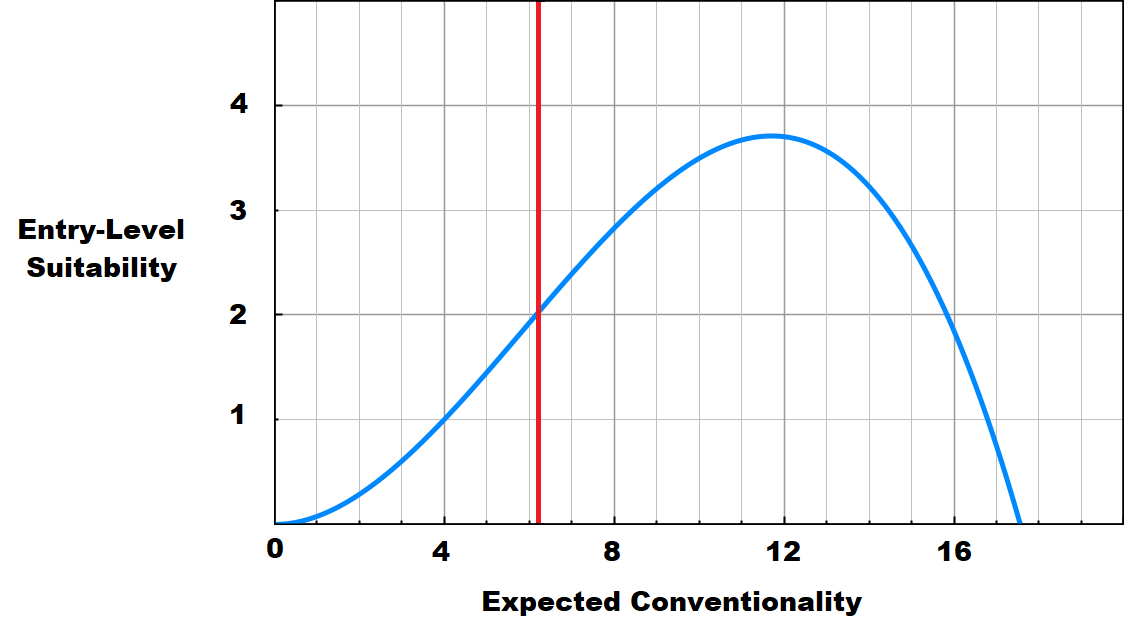
\includegraphics[width=0.9\textwidth]{./figures-and-tables/figure-3.png}
    % \caption{}
    \label{fig:expect_convention_voi}
    \end{figure}

The vertical line in Figure \ref{fig:expect_convention_voi} occurs at the mean value of expected conventionality, or about 6.1.
Alternative credentials are past the lagged phase of adoption and recently past the
point of inflection. Because expected conventionality cannot exceed a value of 10 by
construction, the relation is isomorphic to a sigmoid over the range of actual values.
Log-log regression of conventionalism on time obtains a p-value of .004.
Expected conventionality is not binary,
but a transformed variable was utilized for sigmoid modelling with logistic regression \cite{cox2008stata},
Logistic regression obtained additional significance.

Log-log, s-curve, and sigmoid relations are standard models for a variety of structurally important relationships.
Social learning, experience, social influence, and contagion effects are some of the
indicated structural relations\cite{young2009innovation}.
Further identification of optimal fit may indicate effective accelerators of normalization.

While the relationship between conventionality and time was strong,
this is indirect to the variable of interest. Direct modelling of suitability
on time was insignificant using logarithmic and logistic analysis, but
a two-factor exponential expansion was discovered which forms a useful dynamic model:

\begin{equation} f(x) = b_1b_2^t \end{equation}

This nonlinear model obtained an r-squared of .8691 and $b_2$ had a p-value
less than .001. The estimate of b2 was less than 1, indicating exponential
decay rather than exponential growth. The data indicates a short-run reduction in entry-level
suitability, with comparatively weak evidence for a reversal over time.

When conventionality is interacted with time, a multiple regression suitability on time, conventionality, and the interaction
reveals a positive relation between the interacted variable and suitability.
This may point to long run normalization of alternative credentials as a mechanism toward eventual improvement in entry-level suitability.

While employment status was insignificant in models using data from 2018,
employer effects survived to the preferred 2019 model.
Employer effects are negative in this model, with a coefficient of about -.47.

A simple interpretation is that employers are more pessimistic than others
on alternative credentials. Another interesting possibility is that employer attitude is a leading indicator of population attitude.
Nonlinear regression on time indicates a short-term decline in population favorability,
which is consistent with employer-lead favorability, given that employers are more pessimistic than average in 2019 data.

Exploring this notion, an interesting finding is identified using a multiple regression with interacted time and employer status.
This regression of four parameters on the variable of interest is depicted in
Figure \ref{fig:employer_driven_favorability}, which illustrates a hypothetical reversal in entry-level
suitability. The figure is conceptual and not to scale. The population
trend is illustrated at A, and employer views are represented at B. At A,
time effects are linearly negative and marginally positive. Linear
employer-time effects are positive, but marginal employer-time effects are
negative. The plausibility of a reversal story is enhanced when noting
that the coefficient of interacted manager-time is positive and large in magnitude compared to ordinary time effects.

\begin{figure}[h!]
    \centering
     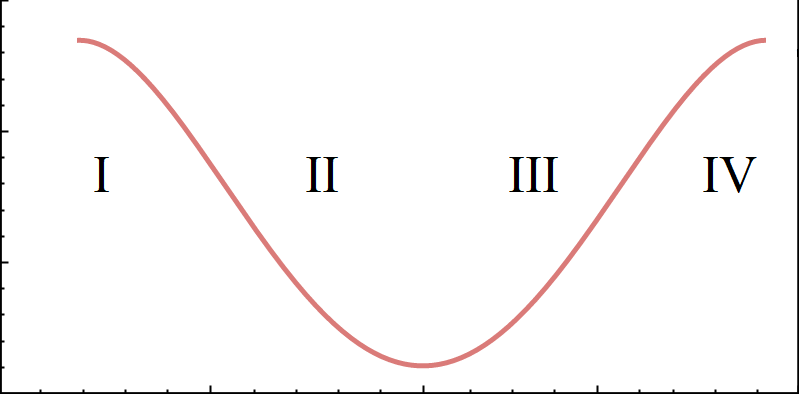
\includegraphics[width=0.9\textwidth]{./figures-and-tables/figure-4.png}
    % \caption{}
    \label{fig:employer_driven_favorability}
    \end{figure}

Age group had a more robust effect compared to exact age, which may
indicate something like a cohort effect. Ethnic effects were moderately
significant, and regional effects continued to be significant after the
introduction of the ethnicity question in 2019, supporting the thesis
that policy differences are important in this regard.

Educational attainment obtained an important effect which was more
significant than either age or income effects. In addition to level of
education, a dummy variable for whether education was at or greater than
obtaining a college degree was found to be significant. Increased
education, whther traditional or non-traditional, appears to be
associated with increased support for alternative credentials.

% TODO: remove from concise paper
\section{Other Interesting Results}

Prior research finds student indifference toward debt\cite{davies1995student}.
The present paper replicates and extends such
findings to identify youth antagonism to alternative credentials. Prior
research often measures debt attitudes among college students, but such
evidence is susceptible to selection bias because debt-tolerant
individuals might have a propensity to consume higher education. In
contrast, the present paper identifies generalized youth antagonism to
alternative credentials.

In a simple regression, age has a small negative coefficient.
Table \ref{tab:partial_crosstab_voi_agegroup} tells a more complex story.
The most positive group is not the youngest group, but the age group actively
attending or having just graduated college.

\begin{table}
    \caption{Partial Crosstab of Age Group on Suitability}
    \begin{tabular}{lllllll}
        Suitability & $<$18 & 18-29 & 30-44 & 45-60 & 60$<$ & Total \\
        1 & 3 & 9 & 11 & 13 & 4 & 40 \\
        5 & 1 & 28 & 31 & 27 & 9 & 96 \\
        10 & 1 & 46 & 39 & 36 & 19 & 141 \\
        Total & 10 & 227 & 250 & 245 & 77 & 809 \\
        Average & 4.60 & 6.93 & 6.62 & 6.40 & 6.34 & 6.59 %
    \end{tabular}
    \label{tab:partial_crosstab_voi_agegroup}
    \end{table}

Minors are the only age group which is unfavorable toward alternative credentials on average.
Minors have the largest share of minimum-favorability responses.
Minors are also the least sampled group in this data set.

In the preferred model and several others, educational effects are important, including a
dummy variable for having received a college-level or better education.
One explanation is that participation in the traditional higher education
drives support for alternative credentials, and the relationship with age is a
side effect.

An interesting, tangential result is the effect of nonbinary gender identification.
Nonbinary gender identification, obtained for 16 respondents, was included in order to
reduce noise on gender effects, but it turned out to have a significant independent effect.

Simple regression of nonbinary gender identification on the variable of
interest reveals a coefficient of about -1.3 with a p-value less than .05.
Substituting nonbinary identification in for other gender variables in the strong model
maintains the negative direction of effect, but the effect is
attenuated to a coefficient of -.48 and a p-value of .374.

\section{Applications}

Results have key applications for employers, students, and policy.
Age results indicate an alternative credential marketing strategy targeted at
current college students, recent graduates, and parents, rather than high school students.

Employers tend to adopt practices supported by leaders in their own industry.
This paper suggests that employers may be a leading indicator of broader attidudes.
Given these two facts, a strategy for social adoption would be to target industry leaders.
At the same time, we already see industry leaders disavowing the need for formal education.
Glassdoor notes 15 leading companies, including Google, which no longer required a degree\cite{glassdoor_2018}. Glassdoor
states, "Increasingly, there are many companies offering well-paying jobs
to those with non-traditional education or a high-school diploma."

% TODO: may not need this paragraph
In 2013, Laszlo Bock, Senior Vice President at Google, stated that Google’s data at that time indicated
that on the job performance was insignificantly related to GPA or test
scores after 2-3 years, and the proportion of people without any college
education at Google was increased over time\cite{bryant_2013}.

For the corporate intrapreneur, direct appeal to industry leaders is one strategy.
Another strategy is simply continued socialization of the topic within the organization.
Results indicate that people are receptive to alternative education even if they aren’t
familiar with the topic, and they become more favorable as they learn
more\footnote{Technically, `reg voi cprovider1` indicates that when a person doesn’t know of any alternative learning providers, there is still a constant of 6.4 in the simple linear regression, indicating positive favorability to the variable of interest. In addition, cprovider1 itself has a significant, positive effect, indicating that informing a person about an alternative learning provider is expected to have a positive impact to the variable of interest, which is alternative credential favorability.}.
A third strategy is to appeal to the underlying costs and benefits of an alternatively educated labor force.
Alternatively educated students tend to be more diverse\cite{florentine_2018}, and improving diversity is often a corporate goal in itself.
Alternatively educated students are also often willing to take a lower starting salary during the junior phase of their career, while providing similar or superior technical output.

Students should consider conducting learning online, learning with non-elite providers,
and leveraging credit by examination.
For roles where a degree is inessential to junior placement, students should consider
deferring college education until after industry employment is obtained.
Once a student obtains employment in the industry, employers are often willing to pay the majority of a reasonably priced degree.
This deferred degree strategy is a key way for a student to obtain a much better return on investment to their education than they otherwise would.
Finally, students should consider leveraging digitial portfolios as a compliment to their degree,
as a means of earning college credit through a prior learning assessment,
and even as a substitute for the degree with respect to particular roles.

Results for policymakers indicate redirecting or limiting federal grant and loan programs.
Licenses which require formal education should be amended to support evidence-based competency in lieu of accredited education.
Internship rules should be relaxed and the minimum wage should be frozen or reduced,
to support better employment of young and concurrently learning individuals.
Finally, tax write-offs and tax-privileged
investment vehicles targeted at accredited education should be liberalized
to support alternative education.

% ref: https://www.youtube.com/watch?v=KS9GvK7cvmo
% https://tex.stackexchange.com/a/51501/197312
\bibliographystyle{/Users/zyl357/Documents/GitHub/research-dissertation-case-for-alt-ed/papers/alt-ed-survey/aea-latex-templates/aea}
\bibliography{BibFile}

\end{document}
